%% Shared article body for paper.tex (styled) and paper-springer-template.tex.

\section{Introduction}\label{sec1}

Since \citet{markowitz1952}, portfolio selection has been treated as a trade-off between expected return and variance, and the Sharpe ratio is still the summary statistic most investors quote \citep{sharpe1966}. Putting the theory to work has proved harder. Optimisers magnify errors in their inputs \citep{michaud1989}, and sixty years of refinements have reduced the problem without removing it \citep{kolm2014}. Machine learning reopened the question because flexible models might forecast those inputs better \citep{gu2020,fischer2018}.

Several recent studies go further and chain learned components into a single pipeline, with clustering choosing the assets, a deep network forecasting their returns and a metaheuristic allocating capital. Each stage has settings to tune, but the whole pipeline is usually judged on one backtest. Empirical finance has repeatedly found large gaps between reported and reproducible performance in designs of this kind \citep{bailey2014pseudo,harvey2016,hou2020}.

\citet{dastkhan2026}, published in \textit{Annals of Operations Research}, is a prominent example. Their framework groups 88 Nasdaq stocks with fuzzy clustering, keeps one representative per group, forecasts each representative's next-month price with an LSTM network, and sets weights with a genetic algorithm that maximises the Sharpe ratio. Over the twelve months of 2024 they report that \$1,000 grew to \$5,344 after transaction costs, with a Sharpe ratio of 11.93 against 0.35 for the Nasdaq Composite and 0.31 for the Nasdaq-100. Three alternative models, each removing one module, are used to argue that every module contributes on its own.

We put these conclusions through four tests. The first asks whether the published figures agree with one another, and the second whether the forecasts carry any skill. The third measures how much of the headline result comes from choices made after seeing the test year. The fourth checks whether the conclusions hold over a longer period when the configuration is chosen out of sample. For this we use the paper's own tables, the 85 stocks of its universe that can still be downloaded, its transaction-cost rule and a reconstruction of its pipeline. Hypotheses, designs and decision rules were committed to a version-controlled repository before any of the corresponding computations ran.

The audit of the published performance table (Section~\ref{sec5.1}) finds two arithmetic inconsistencies, and both widen the framework's apparent lead over its benchmarks. The reported forecast accuracy is no better than a random walk, and over 2018--2024 the forecasts tell us nothing about which stocks will do better next month (Section~\ref{sec5.2}). Choosing the configuration on the test year roughly doubles the 2024 result, which we show with previous-year selection, a random-selection null and the probability of backtest overfitting (Section~\ref{sec5.3}). Finally, a six-year rerun of the paper's own decomposition, with the configuration re-chosen each January, shows that the pipeline's high returns come with correspondingly high risk (Section~\ref{sec5.4}).

Section~\ref{sec2} reviews related work. Section~\ref{sec3} summarises the framework under study and Section~\ref{sec4} describes the data and replication design. Section~\ref{sec5} presents the results, Section~\ref{sec6} discusses them, Section~\ref{sec7} sets out the limitations and Section~\ref{sec8} concludes.

\section{Literature review}\label{sec2}

\subsection{Machine learning for portfolio construction}

Machine learning entered empirical asset pricing on a large scale when \citet{gu2020} compared trees, boosted ensembles and neural networks for return prediction and found economically meaningful gains, concentrated in nonlinear interactions among predictors. Recurrent networks followed soon after, and \citet{fischer2018} showed that LSTM networks \citep{hochreiter1997} could rank daily stock returns better than memory-free classifiers, although the advantage faded in later years of their sample. A systematic review by \citet{novykov2025} maps the deep-learning portfolio literature and notes that many studies rely on a single market and test period.

Work published in 2025 and 2026 extends these ideas in several directions. Reinforcement learning has become a common choice. \citet{xue2026} add attention mechanisms to a reinforcement-learning allocator, and \citet{pavithra2026} give the agent memory so that it can account for path-dependent transaction costs. \citet{zepeda2026} use a transformer-based Q-learning agent for cryptocurrency portfolios, and \citet{huang2026} adapt deep reinforcement learning to long--short portfolios. On the optimisation side, \citet{garg2026} use deep neural networks to build data-driven uncertainty sets for robust portfolio optimisation. These studies share the base paper's ambition of replacing hand-specified inputs with learned ones, and most share its reliance on a small number of backtests.

\subsection{Clustering for asset selection}

Grouping similar assets before allocating capital is an old idea. \citet{nanda2010} applied it to Indian stocks, \citet{long2014} paired clustering with multi-objective optimisation, and \citet{khan2022} clustered stocks on technical-analysis features to build dynamic portfolios. Hierarchical risk parity \citep{lopezdeprado2016} allocates along a tree of correlations and never inverts a covariance matrix. Clustering remains central in recent work. \citet{zouaghia2025} combine K-means with mean--variance optimisation and reinforcement learning, and \citet{ashrafzadeh2025} find that clustering stocks before training improves return forecasts. \citet{ebrahimi2026} use clusters to make cardinality-constrained optimisation tractable, while \citet{dastkhan2026crypto} apply the same family of methods to cryptocurrency portfolios. The hybrid fuzzy C-means of the base paper \citep{bezdek1984} sits in this tradition. Our question is narrower than whether clustering helps diversification in general; we ask whether the particular gains reported for this framework can be reproduced.

\subsection{Estimation risk and benchmarks}

Mean--variance optimisers treat estimated inputs as if they were true, so small errors in expected returns produce large and unstable positions \citep{michaud1989}. Shrinking the covariance matrix towards a structured target \citep{ledoit2004}, or using nonlinear shrinkage of its eigenvalues \citep{ledoit2020}, reduces the damage. Even so, \citet{demiguel2009} find that the naive $1/N$ portfolio is hard to beat out of sample, because the error in estimated means swamps the gains from optimisation. Return predictability is itself fragile, and \citet{welch2008} show that many predictors that work in-sample fail out of sample. Genetic algorithms entered portfolio optimisation through cardinality-constrained problems such as those of \citet{chang2000}, where exact methods become impractical. Any claim of superior performance should therefore be judged against equal weighting and the market index, after costs and on data that the model has not seen.

\subsection{Backtest overfitting and multiple testing}

If many variants of a strategy are tried and only the best is reported, the reported backtest will overstate what an investor can expect. \citet{bailey2014pseudo} show how quickly the best in-sample Sharpe ratio rises with the number of trials, and \citet{bailey2014deflated} propose a deflated Sharpe ratio to correct for it. \citet{bailey2017pbo} go a step further and estimate the probability of backtest overfitting by combinatorially symmetric cross-validation. Formal tests for data snooping come from \citet{white2000} and \citet{hansen2005}, and \citet{harvey2016} argue that a new return predictor should clear a $t$-statistic of about three. Short samples add their own noise. Using the results of \citet{lo2002}, a monthly Sharpe ratio estimated from twelve returns, the length of the base paper's test, has a standard error of roughly 0.3. Large-scale replications point the same way: \citet{hou2020} find that most of 452 published anomalies disappear once microcaps are treated consistently.

\section{The framework under study}\label{sec3}

We summarise \citet{dastkhan2026} as published. The data are 88 Nasdaq-listed stocks with complete daily records from January 2017 to December 2024. Testing covers January to December 2024, and the portfolio is rebuilt each month on an expanding window that begins in January 2017.

In the clustering module each stock is described by its historical mean daily return and daily standard deviation, and the stocks are grouped by fuzzy C-means \citep{bezdek1984} with K-means++ initialisation and Mahalanobis distance. One representative is then picked from each cluster, by maximum return, maximum Sharpe ratio or minimum risk. The number of clusters (two to eight) and the selection criterion are set by comparing how much money each combination has made by the end of the 2024 test year. The forecasting module trains an LSTM network \citep{hochreiter1997} with two layers of 50 units to predict daily prices for the coming month from the two inputs ranked highest by SHAP analysis. The paper reports an average MAPE of 1.67\% for these forecasts. In the allocation module a genetic algorithm maximises expected return per unit of risk. Short sales are excluded and zero weights allowed, and the algorithm runs ten times a month with a population of 50 over 100 generations, mutating each weight with probability 0.05 by Gaussian noise of standard deviation 0.05. Transaction costs of 0.1\% on purchases and 0.2\% on sales are charged on the whole portfolio every month.

The best reported configuration, four clusters with maximum-return representatives, turns \$1,000 into \$5,344. Three alternative models replace clustering with random selection (Alternative Model 1), forecasts with historical means (Alternative Model 2) and optimisation with equal weights (Alternative Model 3), and paired $t$-tests on cumulative returns favour the full model in every comparison.

\section{Data and replication design}\label{sec4}

\subsection{Data}

We collect daily adjusted closing prices from Yahoo Finance for the 88 stocks listed in Appendix~1 of \citet{dastkhan2026}, from January 2017 to December 2024. Three of them (ANSS, EA and WBD) have since been delisted or acquired, which leaves 85. For these 85 stocks, our daily mean returns and standard deviations agree with the paper's Appendix~1 to median absolute differences of 0.00016 and 0.00046. QQQ stands in for the Nasdaq-100 in the backtests, and the index series \textasciicircum{}NDX and \textasciicircum{}IXIC are used for the audit.

\subsection{Reconstruction of the pipeline}

Where the published description is silent we made four choices. Mahalanobis fuzzy C-means is run as ordinary fuzzy C-means on the mean and standard deviation after whitening them by their covariance matrix, which gives the same result. Our forecaster differs most from the original. It is a single LSTM with 16 units shared across stocks, retrained each month on the previous 504 trading days to predict the next 21-day return from the last 60 daily returns. The paper's per-stock price models with SHAP-based feature selection are not described in enough detail to copy, and Section~\ref{sec7} considers what this changes. Risk is the sample covariance matrix of all daily returns since January 2017, and the genetic algorithm uses the published settings without modification. LSTM initialisation, clustering, the genetic algorithm and random selection all depend on random numbers, so every experiment is repeated over five seeds. The code runs in Python~3.13 with NumPy, SciPy, pandas and PyTorch. A full six-year run of the five pipelines takes about 31 minutes per seed on a 12-core laptop, most of it spent retraining the LSTM each month.

\subsection{Pre-registration and statistics}

Every analysis was written into a protocol and committed before it ran. The two clarifications added later were logged before any result was seen. Sharpe ratios are monthly mean returns divided by their standard deviation and scaled by $\sqrt{12}$, with a zero risk-free rate \citep{sharpe1966}. We compare strategies with one-sided $t$-tests on monthly return differences, in the spirit of \citet{diebold1995}, with heteroskedasticity- and autocorrelation-consistent standard errors \citep{newey1987}. A hypothesis is counted as supported when the median $p$-value across seeds is below 0.05 and at least three of the five seeds agree in sign. Holm-adjusted $p$-values are reported next to the raw ones.

\section{Results}\label{sec5}

\subsection{Consistency of the published performance table}\label{sec5.1}

Table~\ref{tab1} compares the annual returns reported by \citet{dastkhan2026} with the returns implied by the final wealth that the same tables report.

\begin{table}[ht]
\caption{Reported annual return against the return implied by the reported final wealth (\$1,000 start)}\label{tab1}
\begin{tabular*}{\textwidth}{@{\extracolsep{\fill}}lrrrr@{}}
\tabletoprule
\tabhead{Row (table in the\\original paper)} & \multicolumn{1}{l}{\tabhead{Reported\\return (\%)}} & \multicolumn{1}{l}{\tabhead{Implied by\\wealth (\%)}} & \multicolumn{1}{l}{\tabhead{Reported\\Sharpe ratio}} & \multicolumn{1}{l}{\tabhead{Reported return\\$\div$ reported risk}} \\
\midrule
Model, maximum return (T7) & 565.89 & 434.4 & 11.93 & 11.93 \\
Model, maximum Sharpe ratio (T7) & 388.45 & 295.8 & 8.95 & 8.95 \\
Model, minimum risk (T7) & 178.26 & 134.5 & 6.65 & 6.65 \\
Alternative Model 1 (T10) & 189.00 & 136.9 & 6.20 & 5.91 \\
Alternative Model 2 (T10) & 23.61 & $-0.05$ & 0.59 & 0.59 \\
Alternative Model 3 (T10) & 88.14 & 55.9 & 2.74 & 2.74 \\
Nasdaq Composite (T7) & 1.37 & 30.4 & 0.35 & 0.35 \\
Nasdaq-100 (T7) & 1.23 & 26.6 & 0.31 & 0.31 \\
\botrule
\end{tabular*}
\end{table}

The first problem lies in Eqs.~14--15 of the original paper, which compound the arithmetic mean monthly return as $(1+\bar R)^{12}-1$. That figure exceeds the realised compound return whenever returns vary, so every model row reports more than its own wealth implies. The gap widens with volatility and therefore flatters the volatile model portfolios more than the benchmarks. Alternative Model 2 is the starkest case. It reports a 23.6\% annual return yet ends the year with slightly less money than it started with.

The second problem is that the benchmark rows use different units. Their reported annual returns of 1.37\% and 1.23\% cannot be reconciled with their own final wealth (+30.4\% and +26.6\%), while their reported annual risk of 3.9--4.0\% is close to the indices' \textit{monthly} volatility in 2024. Table~\ref{tab2} recomputes both benchmarks from 2024 index data.

\begin{table}[ht]
\caption{The 2024 benchmarks recomputed from index data}\label{tab2}
\begin{tabular*}{\textwidth}{@{\extracolsep{\fill}}lrrrrrr@{}}
\tabletoprule
Index & \multicolumn{1}{l}{\tabhead{Monthly\\mean (\%)}} & \multicolumn{1}{l}{\tabhead{Monthly\\s.d. (\%)}} & \multicolumn{1}{l}{\tabhead{2024\\return (\%)}} & \multicolumn{1}{l}{\tabhead{Wealth after\\costs (\$)}} & \multicolumn{1}{l}{\tabhead{Sharpe,\\Eq.~15}} & \multicolumn{1}{l}{\tabhead{Standard\\Sharpe}} \\
\midrule
Nasdaq Composite & 2.18 & 3.35 & 28.6 & 1,241 & 2.54 & 2.16 \\
Nasdaq-100 & 1.92 & 3.22 & 24.9 & 1,205 & 2.30 & 1.98 \\
\botrule
\end{tabular*}
\end{table}

Put on consistent units, the published comparison of 11.93 against 0.31, a ratio of 38 to 1, becomes 11.93 against 2.30 under the paper's own formula. Under the standard Sharpe ratio, recovered from the moments the paper reports, it becomes 4.33 against 1.98. An advantage of about two to one is still large, but it rests on twelve months of data (Section~\ref{sec5.3}).

\subsection{Forecasting skill}\label{sec5.2}

For the same 85 stocks in 2024, a random walk that predicts each day's price as the previous day's has a MAPE of 1.38\%, lower than the 1.67\% reported for the LSTM. For Amazon, the example the paper plots, the random walk scores 1.32\% against a reported 1.33\%. The paper does not say over what horizon its MAPE was measured. Genuine month-ahead price paths with 1.67\% error would beat the month-ahead random walk (4.79\%), but nothing in the paper shows that the forecasts were of that kind. In any case price levels move slowly from day to day, so a low price-level MAPE says little about the value of a forecast for portfolio choice.

For allocation, what matters is whether the forecasts rank next month's returns correctly. Over 84 monthly rebalances from 2018 to 2024, the rank correlation between our LSTM's forecasts and realised returns (the information coefficient) averages between $-0.009$ and $+0.005$ depending on the seed. No seed comes close to significance (all one-sided $p>0.4$). These are our forecasts, not the original ones. The paper, however, reports no accuracy measure on returns, so its claim that the LSTM improves return forecasting rests on price-level fit alone. A near-zero information coefficient is also in line with the broader evidence on out-of-sample return predictability \citep{welch2008}.

\subsection{Choosing the configuration on the test year}\label{sec5.3}

The original paper picks the number of clusters and the representative criterion, 21 combinations in all, by final wealth over 2024, which is also its test year. In its Table~6, final wealth across the combinations ranges from \$1,793 to \$5,344. We reran the 2024 protocol under two selection rules (Table~\ref{tab3}).

\begin{table}[ht]
\caption{Final wealth in 2024 from \$1,000 (mean over five seeds)}\label{tab3}
\begin{tabular*}{\textwidth}{@{\extracolsep{\fill}}lrr@{}}
\tabletoprule
 & \multicolumn{1}{l}{\tabhead{Configuration chosen on\\2024 (as published)}} & \multicolumn{1}{l}{\tabhead{Configuration chosen on\\2023, applied to 2024}} \\
\midrule
Reconstruction of the pipeline & 2,543 & 1,201 \\
QQQ, same costs & -- & 1,211 \\
Equal weight, 85 stocks & -- & 1,121 \\
Published result & 5,344 & -- \\
\botrule
\end{tabular*}
\end{table}

Selecting on the test year roughly doubles the outcome. Selected on 2023 instead, the pipeline ends 2024 level with the Nasdaq-100. Even with selection on the test year our reconstruction falls well short of the published \$5,344, and its best seed reaches \$3,134.

To see whether the best of 21 configurations beats chance, we repeated the paper's Alternative Model 1 at scale. For each number of clusters we drew 100 random-selection paths per seed, with new random stocks every month and the same forecasts and genetic algorithm, and formed the distribution of the best of 21 random configurations. The clustered pipeline's best of 21 beats this null (median $p=0.029$ across seeds), with final wealth of \$2,116--\$3,014 against random medians of \$1,570--\$1,718. Here the original claim holds, since choosing the highest-return representative of each cluster did better than random choice in 2024. Stock-level momentum \citep{jegadeesh1993} offers a simple explanation, because the representative with the highest historical return is usually a recent winner. The published \$5,344 nevertheless lies far beyond anything our reconstruction or its null produced (Fig.~\ref{fig1}).

\begin{figure}[ht]
\centering
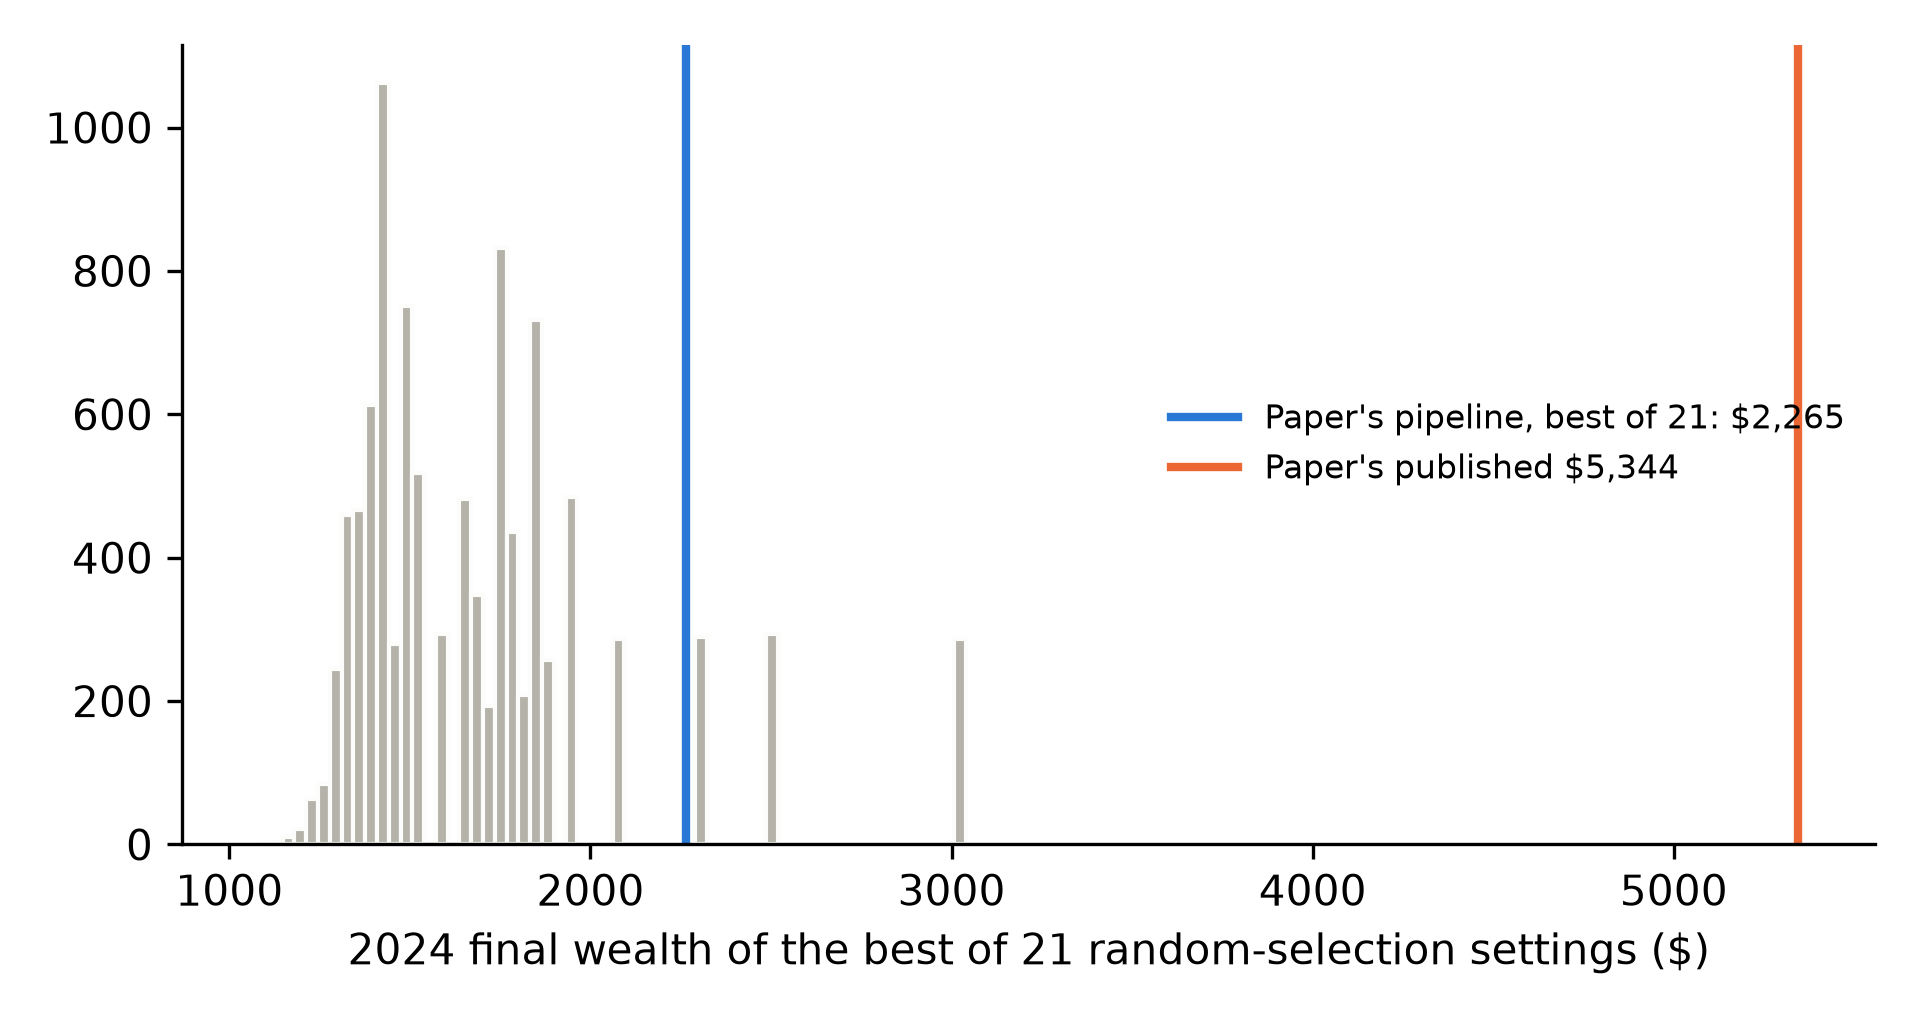
\includegraphics[width=\textwidth]{fig_random_null.png}
\caption{Best of 21 random-selection configurations in 2024 (seed 0), against the reconstruction's best of 21 and the published figure}\label{fig1}
\end{figure}

We also estimated the probability of backtest overfitting over the monthly returns of the 21 configurations from 2018 to 2024, using 924 combinatorially symmetric splits \citep{bailey2017pbo}. PBO ranges from 0.26 to 0.43 across seeds, below the 0.5 that would indicate pure overfitting. Selection therefore carries some information, at a price. The chosen configuration's monthly Sharpe ratio falls by about 40\% out of sample, from 0.41 in-sample to 0.24.

\subsection{Six years with out-of-sample selection}\label{sec5.4}

We extend the test to January 2019--December 2024 (72 months), re-selecting the configuration at the start of each year by the previous year's wealth, and rerun the three alternative models in the same way (Table~\ref{tab4} and Fig.~\ref{fig2}).

\begin{table}[ht]
\caption{2019--2024 with the configuration re-chosen each year on the previous year (five seeds; $\pm$ is the standard deviation across seeds)}\label{tab4}
\begin{tabular*}{\textwidth}{@{\extracolsep{\fill}}lrrr@{}}
\tabletoprule
Pipeline & \multicolumn{1}{l}{\tabhead{Final wealth (\$)}} & \multicolumn{1}{l}{\tabhead{Sharpe ratio}} & \multicolumn{1}{l}{\tabhead{Maximum drawdown (\%)}} \\
\midrule
Original pipeline & 9,569 $\pm$ 4,193 & 0.97 $\pm$ 0.15 & $-44.2$ \\
Alternative 1: random selection & 2,166 $\pm$ 1,097 & 0.48 $\pm$ 0.26 & $-45.3$ \\
Alternative 2: historical means & 5,033 $\pm$ 1,326 & 1.00 $\pm$ 0.16 & $-34.6$ \\
Alternative 3: equal weights & 5,491 $\pm$ 420 & 0.92 $\pm$ 0.03 & $-49.3$ \\
QQQ & 2,776 & 0.93 & $-35.0$ \\
Equal weight, 85 stocks & 3,082 & 1.05 & $-27.4$ \\
\botrule
\end{tabular*}
\end{table}

\begin{figure}[ht]
\centering
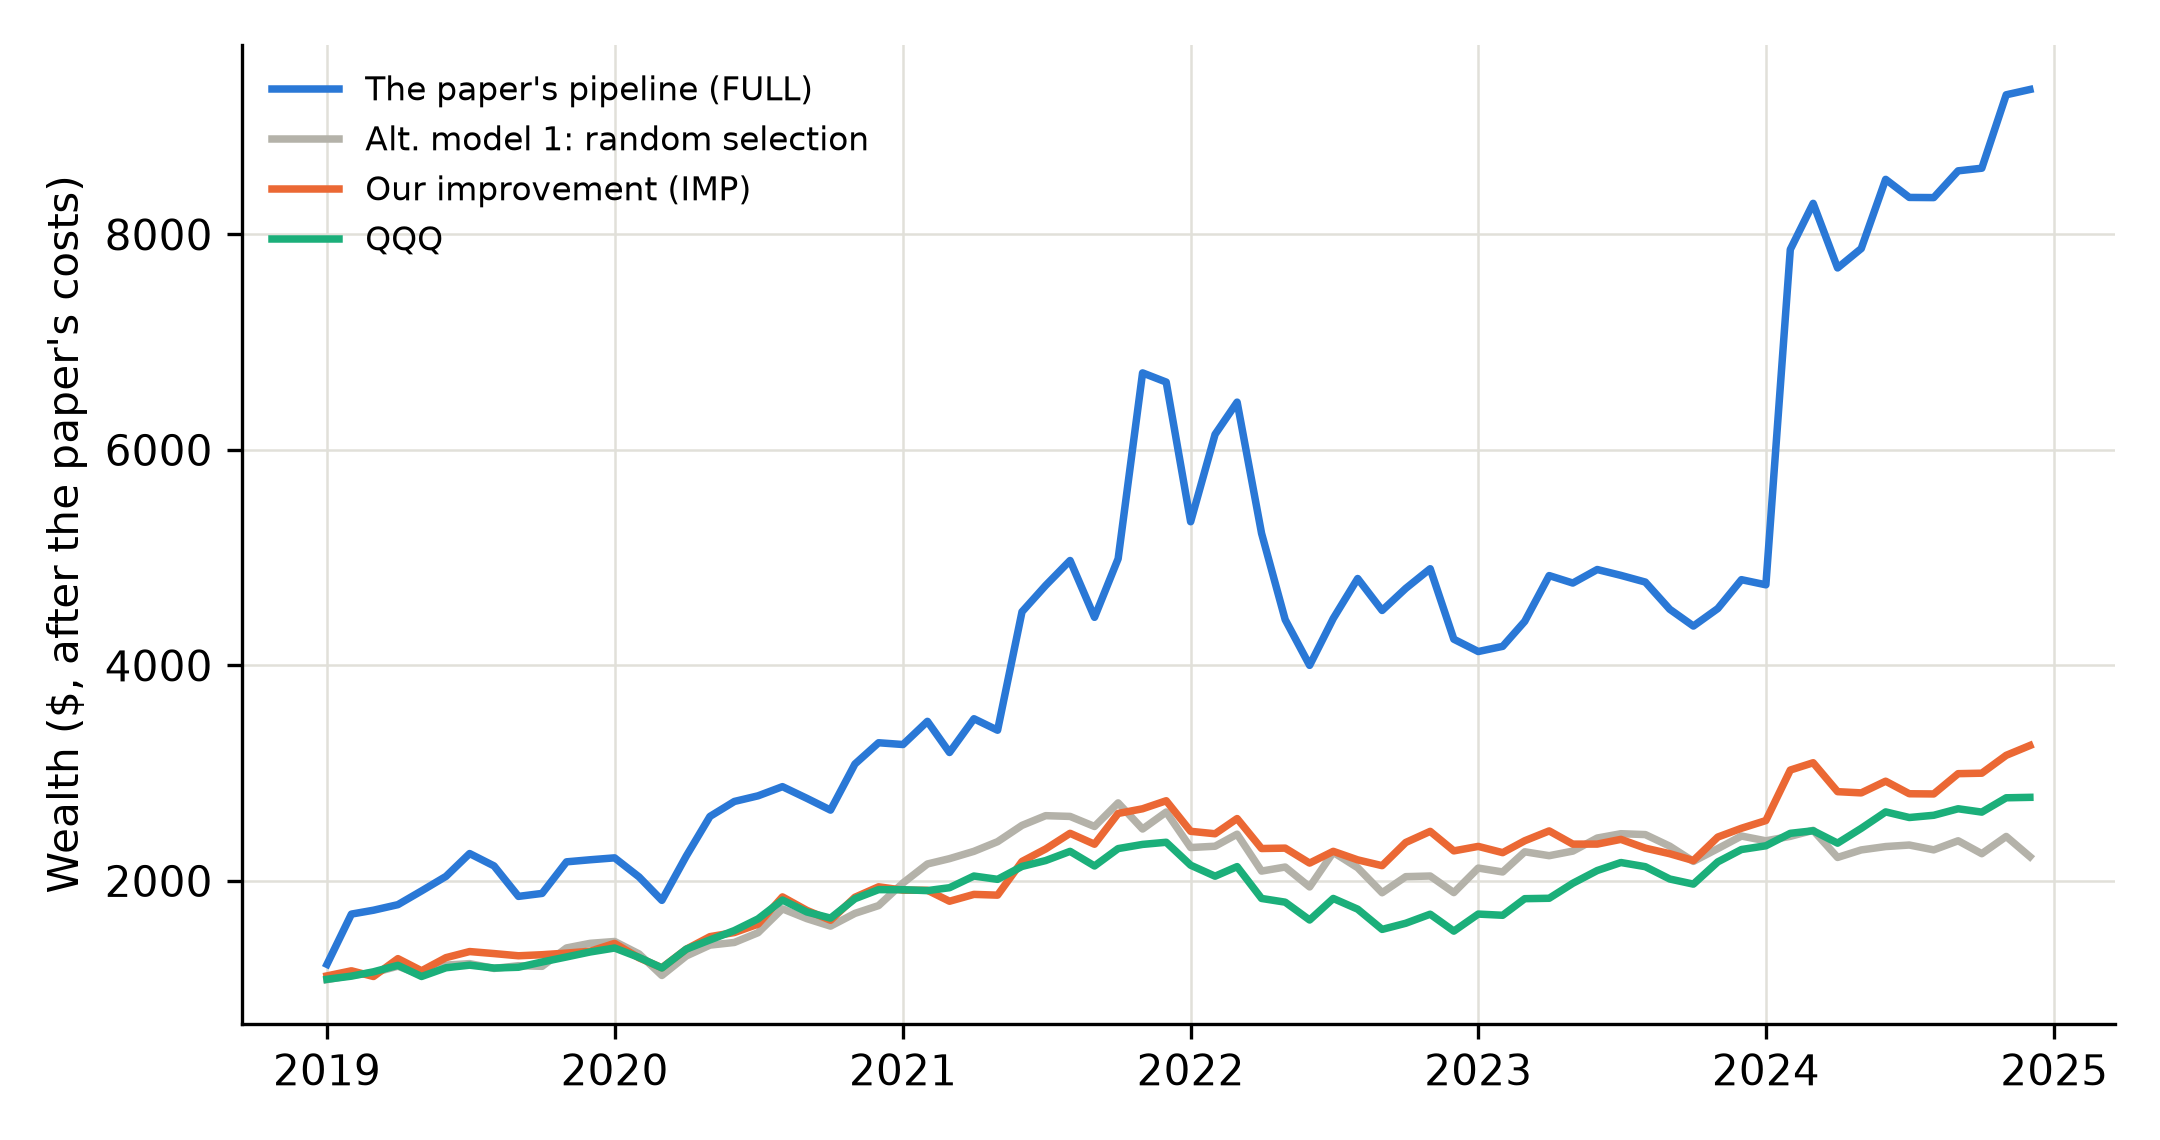
\includegraphics[width=\textwidth]{fig_walkforward_wealth.png}
\caption{Wealth paths from \$1,000, 2019--2024, after the original paper's transaction costs (average over seeds)}\label{fig2}
\end{figure}

The pipeline ends with more than three times the wealth of QQQ, and its risk profile accounts for most of the difference. In an exploratory analysis outside the pre-registered tests, the pipeline holds 3.2 stocks on average, has an annualised volatility of 47.7\% (2.3 times QQQ's 20.6\%) and a beta of 1.10 against QQQ. Per unit of risk it does no better than the market. Its Sharpe ratio of 0.97 compares with 0.93 for QQQ and 1.05 for an equal-weighted portfolio of all 85 stocks, and its maximum drawdown of $-44\%$ compares with $-35\%$ and $-27\%$.

Table~\ref{tab5} tests the paper's decomposition claims over the six years. Each module raises returns in at least four of five seeds, as the paper claims, but none of the differences is statistically significant. The return gaps are large because the strategy is volatile, and the same volatility makes them statistically indistinguishable from zero. Alternative Model 2, which drops the LSTM, has a slightly higher Sharpe ratio (1.00) and a smaller drawdown. This fits the finding of Section~\ref{sec5.2} that the forecasts add risk but no information.

\begin{table}[ht]
\caption{The original paper's decomposition claims, 2019--2024 (HAC $t$-tests on monthly return differences). ``Supported (raw)'' meets the pre-registered rule but not after Holm adjustment}\label{tab5}
\begin{tabular*}{\textwidth}{@{\extracolsep{\fill}}lrrrl@{}}
\tabletoprule
Claim & \multicolumn{1}{l}{\tabhead{Return gap\\(pp per year)}} & \multicolumn{1}{l}{\tabhead{Median $p$}} & \multicolumn{1}{l}{\tabhead{Holm $p$}} & Verdict \\
\midrule
Clustering beats random selection & 30.3 & 0.058 & 0.29 & Not supported \\
LSTM beats historical means & 15.0 & 0.094 & 0.38 & Not supported \\
Genetic algorithm beats equal weights & 11.0 & 0.105 & 0.38 & Not supported \\
Pipeline beats QQQ & 27.4 & 0.038 & 0.23 & Supported (raw) \\
\botrule
\end{tabular*}
\end{table}

\subsection{A diversified variant}\label{sec5.5}

We also tested one improvement, fixed in advance. It keeps three stocks per cluster instead of one, shrinks the forecasts halfway towards their cross-sectional mean, estimates risk with the nonlinear shrinkage of \citet{ledoit2020} and solves the maximum-Sharpe problem exactly with a 30\% cap per stock. Volatility (24.7\%) and drawdown ($-25.0\%$) fell to roughly half, but the Sharpe ratio (0.90) did not rise. The variant did not beat the original pipeline's returns ($p=0.92$), nor QQQ by a significant margin ($p=0.45$).

\section{Discussion}\label{sec6}

Part of the original evidence stands up. Choosing the highest-return stock of each cluster beat random choice in 2024, and over six years the pipeline's returns exceeded the index's in every seed. An investor who wanted concentrated, high-risk exposure to recent Nasdaq winners could have used the framework and would have been paid for that risk over 2019--2024.

The central evidence does not hold up. A Sharpe advantage of 38 to 1 and a five-fold gain in wealth within one year disappear once units are made consistent (Section~\ref{sec5.1}), the configuration is chosen before the test year (Section~\ref{sec5.3}) or the test is extended (Section~\ref{sec5.4}). The forecasts show no skill (Section~\ref{sec5.2}), and over six years none of the module contributions is statistically significant.

As an engineering design the framework is sensible. Its evaluation, though, combined several practices that each favour complex pipelines. The test covered a single year and the configuration was chosen on that year. The headline metric rewards volatility, the benchmark rows used different units, and significance was tested on cumulative returns, which are strongly autocorrelated. None of these practices is rare in the literature, which is one reason replication studies are worth doing. Four simple reporting rules would have caught most of the problems here. Configurations should be chosen only on data from before the test period. The standard Sharpe ratio should be reported, with benchmarks computed by the same code as the strategy. Volatility, drawdown and the number of holdings belong next to returns. And the test should span several years and include an equal-weighted portfolio as well as an index.

\section{Limitations}\label{sec7}

Our forecaster is not the original one. The per-stock price LSTMs with SHAP feature selection are not specified in full and their code is not public. A better forecaster could change the pipeline's absolute performance, but it would leave untouched the audit in Section~\ref{sec5.1}, the selection effect in Section~\ref{sec5.3} and the risk-adjusted comparison in Section~\ref{sec5.4}. We could not reproduce the published \$5,344, which may depend on details we were unable to recover. Three of the 88 stocks are no longer available, and both studies use current constituents and so share survivorship bias. Six years of monthly data give limited statistical power, and comparisons within 2024 alone give very little.

\section{Conclusion}\label{sec8}

Rerun with its own data, costs and design, the framework of \citet{dastkhan2026} earns high returns by holding a few volatile stocks through a strongly rising market. Per unit of risk it does no better than the index or an equal-weighted portfolio, its forecasts show no measurable skill, and its headline figures are inflated by the way returns were computed and configurations chosen. For a portfolio manager the relevant measure is the return a method adds for the risk it takes, with its settings fixed before the test begins. On that measure, simple diversified portfolios remain the benchmark that machine learning frameworks for portfolio management have yet to beat.

\backmatter

\section*{Declarations}

\bmhead{Funding} No funding was received for this study.

\bmhead{Competing interests} The authors have no competing interests to declare that are relevant to the content of this article.

\bmhead{Ethics approval and consent to participate} Not applicable.

\bmhead{Consent for publication} Not applicable.

\bmhead{Data availability} Daily prices were obtained from Yahoo Finance. The list of stocks, all intermediate results and the protocols are available from the corresponding author on request.

\bmhead{Materials availability} Not applicable.

\bmhead{Code availability} The code that produces every number in this article is available from the corresponding author on request.

%% CRediT roles drafted for the team; adjust if anyone's actual work differs.
\bmhead{Author contribution}
\begin{list}{}{\setlength\leftmargin{1em}\setlength\itemindent{-1em}\setlength\itemsep{1.5pt}\setlength\parsep{0pt}\setlength\topsep{3pt}}
\item \textbf{Shivansh Katiyar} (2024IMG-042): conceptualisation; research design and pre-registration protocols; software (pipeline reconstruction and walk-forward backtesting engine); formal analysis; writing (original draft); project administration.
\item \textbf{Neerav Mishra} (2024IMG-029): methodology for statistical inference (heteroskedasticity- and autocorrelation-consistent tests, Holm adjustment, probability of backtest overfitting); validation of results across seeds; writing (review and editing).
\item \textbf{Chandaluri Hemateja} (2024IMG-014): data curation (price collection and reconciliation of the stock universe with the base paper's appendix); investigation (audit of the published performance tables); writing (review and editing).
\item \textbf{Srijan Singh} (2024IMG-046): software (LSTM forecasting module and reproduction of the genetic algorithm); random-selection experiments; validation.
\item \textbf{Tanushri Reddy Dadireddy} (2024IMG-050): literature review and reference verification (cross-checking every citation against its DOI record); investigation (benchmark index data and recomputation of the 2024 Nasdaq benchmarks); random-walk forecast baselines; visualisation (figures and tables); typesetting of the manuscript; writing (review and editing).
\end{list}
\noindent All authors read and approved the final manuscript.

